\sectionquestion{Perceptron}

\begin{parts}
    \part[1] \textbf{True or False:} One difference between batch learning and online learning is that in batch learning, the algorithm has access to labels for all the data points used to train the model while in online learning, the algorithm never sees the true label of a data point.  
    \begin{checkboxes}
        \choice True 
        \choice False
    \end{checkboxes}
    \begin{soln}
        False
    \end{soln}
    \begin{qauthor}
        Henry
    \end{qauthor}
    
    \part[2] \textbf{Short Answer:} Suppose you have a binary classification dataset where the label is either $+1$ or $-1$. The dataset consists of three binary features, $x_1$, $x_2$, and $x_3$, which are all either $0$ or $1$. Furthermore, suppose that the label is $+1$ if two or more of the features have value $1$ and $-1$ otherwise. 
    
    Is this dataset \emph{always} linearly separable? If you answered yes, provide the parameter vector (including a bias term) for a Perceptron that can perfectly classify such a dataset; if you answered no, provide a counterexample in the form of a dataset that satisfies the conditions above which is not linearly separable. 
    
    \begin{tcolorbox}[fit,height=5cm, width=15cm, blank, borderline={1pt}{-2pt}, nobeforeafter=false]
        \begin{soln}
            Yes, such a dataset is always linearly separable and could be perfectly classified by the parameter vector $\thetav=[-1.5, 1, 1, 1]^T$
        \end{soln}
    \end{tcolorbox}
    
    \begin{qauthor}
        Varsha
        
        Edited by Henry
    \end{qauthor}
    
    \part[2] \textbf{Select all that apply:} Suppose you are given a training dataset with two real-valued features $x_1$ and $x_2$ that is \emph{linearly separable}. In this setting, which of the following statement(s) about the batch Perceptron learning algorithm is/are true?
    {%
        \checkboxchar{$\Box$} \checkedchar{$\blacksquare$} % change checkbox style locally
        \begin{checkboxes}
            \choice For any linear decision boundary in this space, there is a single, unique corresponding weight vector i.e., every linear decision boundary can only be represented by one vector. 
            \choice The decision boundary in each iteration of the algorithm can be represented as $\textrm{sign}(w_1x_1+w_2x_2)$ for some coefficients $w_1$ and $w_2$.
            \choice The decision boundary in each iteration of the algorithm is always perfect, i.e., corresponds to a Perceptron with zero training error rate. 
            \choice Once the algorithm has converged, the returned classifier will always be the same, regardless of the order the data points were looped through. 
            \choice None of the above % Keep this option!
        \end{checkboxes}
    }
    \begin{soln}
        E
    \end{soln}
    \begin{qauthor}
        Rohan Chawla, Explain the difference between online learning and batch learning, Determine whether the perceptron algorithm will converge based on properties of the dataset, and the limitations of the convergence guarantees, Describe the inductive bias of perceptron and the limitations of linear models

        Edited by Henry
    \end{qauthor}
    \begin{qtester}
        I don't know if option B was covered in class. I also don't know if this option is strictly not true. 
    \end{qtester}

    \clearpage
    
    \part Suppose you have trained a Perceptron classifier to predict whether or not a given narwhal is Neural (our class mascot) or an imposter, corresponding to labels $y=+1$ and $y=-1$. The inputs to your classifier are two real-valued features, $x_1$ and $x_2$, and your current parameter vector is $\thetav = [2, 2, 1]^T$; note that we are making use of the notational convention presented in lecture where a $1$ is prepended to the feature vectors. 
    
    \begin{subparts}
        \subpart[3] \textbf{Drawing:} On the figure provided below, draw the decision boundary corresponding to your classifier; for full credit, you must clearly indicate the side of the decision boundary that would be classified as $+1$ by writing the words ``Positive'' and ``Negative'' on the figure. 
        
        \begin{center}
        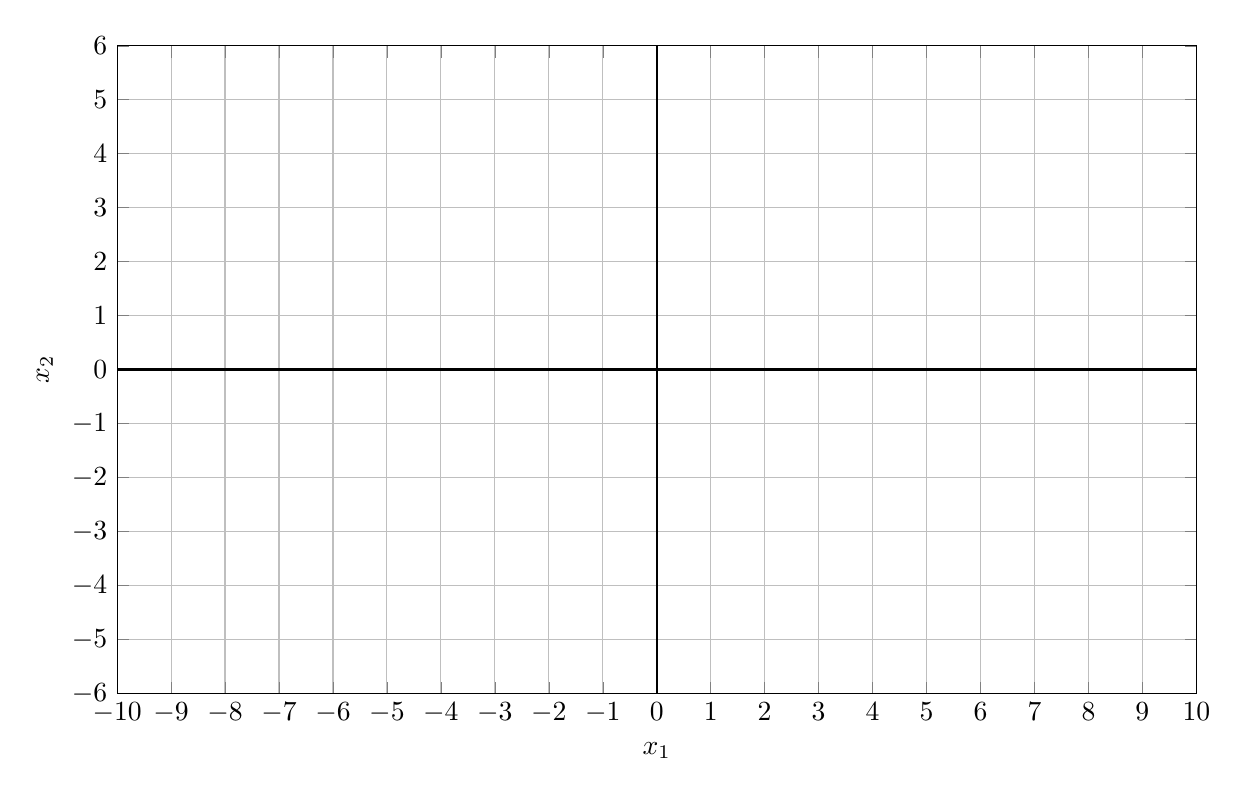
\begin{tikzpicture}
        \begin{axis}[
            scale=2.0, axis equal image,
            xmin=-10, xmax=10, xtick={-10,...,10},
            ymin=-6, ymax=6, ytick={-6,...,6},
            samples=50, grid=major, xlabel=$x_1$, ylabel=$x_2$]
            \addplot [mark=none,  black, thick] coordinates {(-10, 0) (10, 0)};
            \addplot [mark=none,  black, thick] coordinates {(0, -6) (0, 6)};
        \end{axis}
        \end{tikzpicture} 
        \end{center}
        \begin{soln}
            \begin{center}
            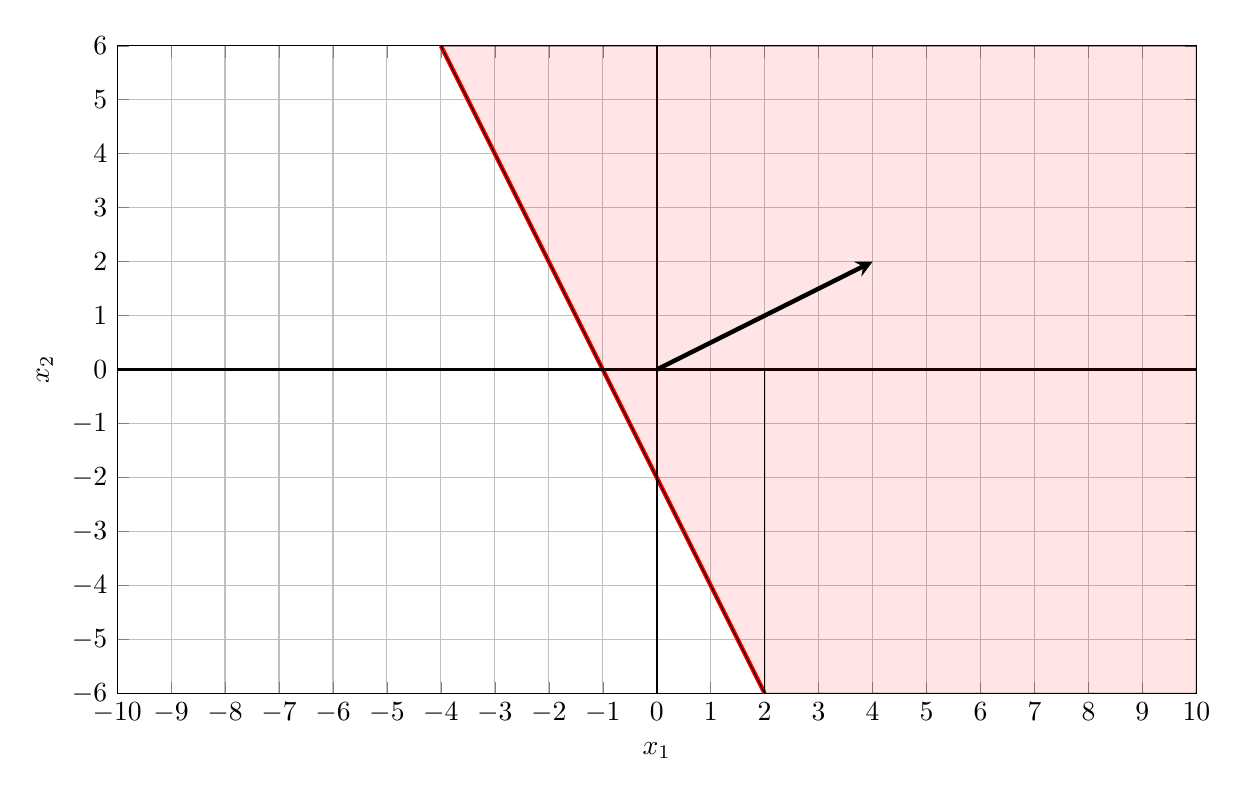
\begin{tikzpicture}
            \begin{axis}[
                scale=2.0, axis equal image,
                xmin=-10, xmax=10, xtick={-10,...,10},
                ymin=-6, ymax=6, ytick={-6,...,6},
                samples=50, grid=major, xlabel=$x_1$, ylabel=$x_2$]
                \addplot [mark=none, red, ultra thick] coordinates {(2, -6) (-4, 6)};
                \addplot [mark=none, black, thick] coordinates {(-10, 0) (10, 0)};
                \addplot [mark=none, black, thick] coordinates {(0, -6) (0, 6)};
                \addplot [fill=red, fill opacity=0.1] coordinates {(2, -6) (10, -6) (10, 6) (-4, 6) (2, -6)} \closedcycle;
                \draw [-stealth, black, ultra thick] (0,0)--(4, 2);
            \end{axis}
            \end{tikzpicture} 
            \end{center}
        \end{soln}
        
        \subpart[2] \textbf{Drawing:} Suppose you realized that you made a computational error during training and the actual parameter vector should be $\thetav' = [\mathbf{1}, 2, 1]^T$. 
        
        On the same figure above, draw an arrow rooted at the origin that points in the direction that you should shift your old decision boundary in order to arrive at the new decision boundary. For full credit, your arrow must be perpendicular to the decision boundary you drew. 
        
        \subpart[1] \textbf{Select one:} Using your new parameter vector, $\thetav' = [1, 2, 1]^T$, how would your classifier classify a narwhal with features $x^{(i)} = [4, -2]^T$?
        \begin{checkboxes}
            \choice $\hat{y}=+1$
            \choice $\hat{y}=-1$
            \choice There is not enough information to compute your classifier's prediction.
        \end{checkboxes}
        \begin{soln}
            A
        \end{soln}
        \begin{qtester}
            I don't think we have introduced any of our mascots, so this is maybe a little hard to parse without insider knowledge. E.g. I don't want someone thinking "Markov clone" is an ML term.
        \end{qtester}
        
        \subpart[2] \textbf{Numerical answer:} Now suppose another narwhal with features $x^{(j)} = [-6, 3]^T$ comes along. Your new classifier predicts their label to be $\hat{y}=-1$ but their true label turns out to be $y^{(j)}=+1$. You update $\thetav'$ based on this new narwhal using the Perceptron learning algorithm: what is your parameter vector after the update? 
    
        $\thetav = $ \begin{tcolorbox}[fit,height=1cm, width=6cm, blank, borderline={1pt}{-2pt}, nobeforeafter=false]
            \begin{soln}
                $[2, -4, 4]$
            \end{soln}
        \end{tcolorbox}
        
        \begin{comment}
            \subpart[2] \textbf{Short answer:} What is the effect of the change in bias term on the decision boundary? Justify why this decreases the mistakes (or errors) that the decision boundary makes.
            \fillwithlines{2em}
            \begin{soln}
                The bias term increased by one, which means that the decision boundary moves toward the negative points, which allows for the positive space to increase and thus allow for potentially more examples with positive labels to be classified correctly.
            \end{soln}
            \begin{qtester}
                The answer you are looking for is very specific. I think most people will just say that the line will no longer pass through the origin. We may want to ask something about in which direction will the line shift
            \end{qtester}
            
            \subpart[2] \textbf{Short answer:} The 10-301 TA team has wants to utilize a fully-converged iteration of this classifier to identify different clones. With the given information, is it guarenteed for the model to converge? Justify your answer.
            \fillwithlines{2em}
            \begin{soln}
                No. If the data is not linearly separable, then it may not be possible to to converge. 
            \end{soln}
        
            \subpart[1] \textbf{Drawing: } Assume that the perceptron algorithm does converge. On the graph below, approximately draw the relationship between total number of mistakes vs. number training examples.
            \begin{center}
            \begin{tikzpicture}
            \begin{axis}[
                scale=1.5, axis equal image, mark options={scale=1.5},
                xmin=0, xmax=6, xtick={1,...,5},
                ymin=0, ymax=6, ytick={1,...,5},
                samples=50, grid=major, xlabel=Examples, ylabel=Total Mistakes]]
                \begin{soln}
                   \addplot[latex-latex,smooth,black,mark=none,%samples=140,
                    line width=1.5pt,domain=-3.5:9.5,
                    samples=63,
                    color=red]  {ln(x)+2};
                \end{soln}
            \end{axis}
            \end{tikzpicture} 
            \end{center}
        
            \begin{qtester}
                Solution needed. This question seems a little tricky to me. 
            \end{qtester}
        \end{comment}   
    \end{subparts}
    \begin{qauthor}
        Sebastian Lu. Draw the decision boundary of a linear model.
        Identify whether a dataset is linearly separable or not. 
        Defend the use of a bias term in perceptron (shifting points after projection onto weight vector). Adapted from 5.4 and 5.5 from F23 exam.
        
        Edited by Henry
    \end{qauthor}

    \part[2] \textbf{Short answer:} Suppose you learn a Perceptron using a linearly separable training dataset and you converge to a classifier that perfectly classifies the training dataset; let the parameter vector you learn be $\hat{\thetav}$. Unfortunately, it turns out you made a mistake when coding your labels: every training data point that you thought had label $+1$ actually had label $-1$ and vice versa. 
    
    Luckily, Neural the narwhal has a simple fix: he tells you that you can compute a new parameter vector $\thetav^*$ that actually correctly classifies the entire training dataset (using the right labels) \emph{without having to retrain}. In 1-2 concise sentences or a single mathematical equation, describe how you could compute $\thetav^*$ using $\hat{\thetav}$.
    \fillwithlines{9em}
    \begin{soln}
        Negate all the weights
    \end{soln}
    \begin{qauthor}
        Varsha, Implement the perceptron algorithm for binary classification

        Edited by Henry
    \end{qauthor}
    
    \part[2] \textbf{Select all that apply:} Suppose you have a linearly separable training dataset, $\mathcal{D}$. Using the Perceptron mistake bound, you compute that the batch Perceptron learning algorithm will make at most $C$ mistakes on $\mathcal{D}$ before converging. Which of the following operations/transformations on the training dataset \emph{could} change this maximum number of mistakes? 
    {%
        \checkboxchar{$\Box$} \checkedchar{$\blacksquare$} % change checkbox style locally]
        \begin{checkboxes}
            \choice Duplicating each data point such that the training dataset now contains $2$ copies of each data point.
            \choice Adding a new feature to every data point that always has value $0$. 
            \choice Rescaling the features by multiplying each feature by $2$. 
            \choice Rotating the entire dataset $4$ degrees around the origin. 
            \choice None of the above
        \end{checkboxes}
    }
    \begin{soln}
        E
    \end{soln}
    \begin{qauthor}
        Henry
    \end{qauthor}

    \begin{comment}
        \part[2] \textbf{Select all that apply:} Which of the following statements is true for the convergence of a perceptron on a binary classification problem:
        {%
        \checkboxchar{$\Box$} \checkedchar{$\blacksquare$} % change checkbox style locally]
        \begin{checkboxes}
            \choice If the batch perceptron learning algorithm converges, the number of mistakes it makes before convergence depends on the order in which data points are seen. 
            \choice Whether or not the batch perceptron learning algorithm converges depends on the order in which data points are seen. 
            \choice The batch perceptron learning algorithm will make a bounded number of mistakes if the training dataset is not linearly separable.
            \choice The batch perceptron learning algorithm will loop forever if the training dataset is not linearly separable.
            \choice None of the above
        \end{checkboxes}
        }
        \begin{soln}
        A - order affects the mistakes the perceptron makes \& D - the perceptron does not converge on data that is not linearly separable.
        \end{soln}
        \begin{qauthor}
        Author: Aditi Sharma
        Objective: Determine whether the perceptron algorithm will converge based on properties of the dataset, and the limitations of the convergence guarantees
        
        Edited by Henry
        \end{qauthor}

        \begin{qtester}
        EA Feedback: I like this question. I wonder if we should specify that there is no stopping condition other than convergence or something. But I also don't want to make it too obvious. 
        \end{qtester}
        
        \part[1] \textbf{True or False:} In classification, online learning differs from batch learning in that the former aims to minimizes the number of mistakes it makes on the training examples, whereas the latter aims to minimize mistakes on a fixed set of held out examples.
            \begin{checkboxes}
             \choice True 
             \choice False
            \end{checkboxes}
            \begin{soln}
            True
            \end{soln}
            \begin{qauthor}
            Matt
            \end{qauthor}
        
        
        \part[4] \textbf{Select all that apply:} Which of the following datasets is linearly separable?
        
        \begin{minipage}{0.3\linewidth}
        \textit{Dataset A:}\\
        \begin{tabular}{ccc}
             $x_1$ & $x_2$ & $y$ \\
             \midrule
             -2 & -2 & -1 \\
             -1 & -1 & -1 \\
             0 & 0 & +1 \\
             1 & 1 & +1 \\
             2 & 2 & +1 \\
        \end{tabular}
        \end{minipage}
        %
        \begin{minipage}{0.3\linewidth}
        \textit{Dataset B:}\\
        \begin{tabular}{ccc}
             $x_1$ & $x_2$ & $y$ \\
             \midrule
             0 & 0 & -1 \\
             1 & 1 & -1 \\
             0 & 1 & +1 \\
             1 & 0 & +1 \\
        \end{tabular}
        \end{minipage}
        %
        \begin{minipage}{0.3\linewidth}
        \textit{Dataset C:}\\
        \begin{tabular}{cccc}
             $x_1$ & $x_2$ & $x_3$ & $y$ \\
             \midrule
             2 & 0 & 0 & -1 \\
             3 & 1 & 1 & -1 \\
             2 & 1 & 0 & -1 \\
             1 & 0 & 3 & +1 \\
             1 & 2 & 1 & +1 \\
             2 & 2 & 2 & +1 \\
        \end{tabular}
        \end{minipage}
            {%
            \checkboxchar{$\Box$} \checkedchar{$\blacksquare$} % change checkbox style locally
            \begin{checkboxes}
             \choice Dataset A
             \choice Dataset B
             \choice Dataset C
             \choice None of the above
            \end{checkboxes}
            }
            \begin{soln}
            Dataset A and Dataset C
            \begin{itemize}
                \item A: really just a line (extra feature is a copy)
                \item B: XOR
                \item C: example solution $\wv = [-1, 1, 1], b = 0$
            \end{itemize}
            Points: correctness on A is worth 1 pt, correctness on B is 1 pt, correctness on C is 2 pts.
            \end{soln}
            \begin{qauthor}
            Matt
            \end{qauthor}
        
        \clearpage
        
        \part Suppose you are given a linear decision boundary defined by weight vector $\wv = [10, -8]^T$ and intercept $b = 0$. \emph{(Note: For each question below, draw your answer on the provided axes and clearly label each part.)}
        
        %\begin{figure}[H]
            \begin{center}
            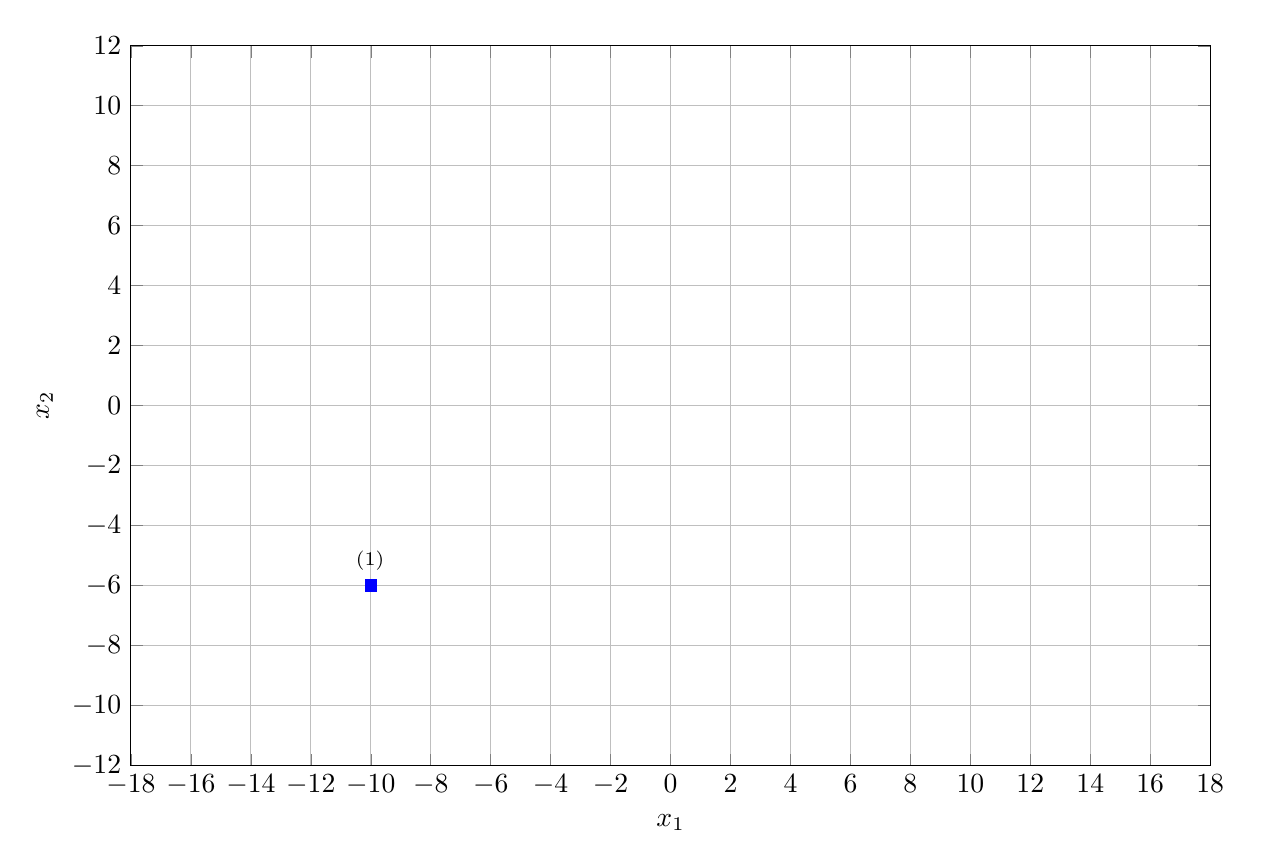
\begin{tikzpicture}
            \begin{axis}[
                scale=2.0, axis equal image,
                xmin=-18, xmax=18, xtick={-18,-16,...,18},
                ymin=-12, ymax=12, ytick={-12,-10,...,12},
                samples=50, grid=major, xlabel=$x_1$, ylabel=$x_2$]
                %\addplot[blue, ultra thick] (x,x*x);
                %\addplot[red,  ultra thick] (x*x,x);
                \addplot [
                    scatter,
                    only marks,
                    point meta=explicit symbolic,
                    scatter/classes={
                        a={mark=square*,blue},
                        b={mark=triangle*,red}
                    },
                    nodes near coords*={$\xv^{(\pgfmathprintnumber[frac]\myvalue)}$},
                    visualization depends on={\thisrow{myvalue} \as \myvalue},
                ] table [meta=label] {
                    x y label myvalue
                    -10 -6 a 1
                };
            \end{axis}
            \end{tikzpicture}
            \end{center}
           % \caption{}
        %    \label{fig:percdata}
        %\end{figure}
        
        \begin{subparts}
        
        \subpart[1] Draw the weight vector $\wv$.
        
        \subpart[2] Draw the decision boundary.
        
        \subpart[1] \textbf{Select one:} Would this classifier correctly or incorrectly classify the point shown as $\xv^{(1)}$ if its true label is $y^{(1)} = +1$?
            \begin{checkboxes}
             \choice correctly classify
             \choice incorrectly classify
            \end{checkboxes}
            \begin{soln}
            Incorrectly classify
            \end{soln}
            \begin{qauthor}
            Matt
            \end{qauthor}
        
        \subpart[2] Suppose the intercept $b$ is decreased to some new value such that $b < 0$. Draw an arrow pointing in the exact direction that the decision boundary will move, relative to its current position.
            \begin{soln}
            Arrow pointing down and/or right (in the direction of w)
            \end{soln}
            \begin{qauthor}
            Matt
            \end{qauthor}
        \subpart[2] Briefly justify why, in a Perceptron, subtracting one from the value of $b$ when we make a mistake and the label is negative is a sensible adjustment to the parameters.
            \fillwithlines{6em}
            \begin{soln}
            Subtracting one will move the decision boundary towards (the avg. of) those positive points on which Perceptron previously made a mistake and away from (the avg. of) those negative points on which it made mistake, thus creating more space on the negative side relative to the previous decision boundary before said intercept adjustment.
            \end{soln}
            \begin{qauthor}
            Matt
            \end{qauthor}
        \end{subparts}
    \end{comment}
\end{parts}